\section{Resoconto delle attività di verifica}
\label{resoconto}
\subsection{Periodo di analisi}
Durante questo periodo, i documenti redatti da presentare in ingresso alla \glo{\textbf{RR}} sono stati verificati dai \textit{Verificatori} secondo i criteri per l'analisi statica definiti nelle \NdPv{2.0}, seguendo le metodologie di \glo{Walkthrough} e di \glo{Inspection}.
\subsubsection{Strategia adottata per l'analisi statica}
Per ciascun documento si è creato inizialmente una struttura di base comune così da evitare possibili conflitti e sprechi di tempo futuri. A questo punto si è applicato il metodo del Walkthrough sulla parte di documento modificata che ha permesso l'individuazione di errori comuni e frequenti all'interno dei documenti che hanno comportato un aggiornamento della lista di controllo. Si è potuto infatti svolgere un'ulteriore esame nei confronti del documento sottoposto a verifica per scoprire gli errori non visti nelle verifiche precedenti tramite un'\glo{attività} di Inspection. Il \textit{Verificatore} valuta la correttezza del documento cercando di individuare eventuali errori e trattandoli nel modo seguente:
	\begin{itemize}
		\item Correzione degli errori ortografici e sintattici o di eventuali violazioni delle norme tipografiche stabilite nelle \NdPv{3.0};
		\item Inserimento degli errori più ricorrenti nella lista di controllo, redatta durante la \glo{fase} di verifica dei documenti;
		\item Applicazione del ciclo PDCA per migliorare e velocizzare le verifiche future.
	\end{itemize}
\subsubsection{Strategia adottata per l'analisi dinamica}
L'analisi dinamica di ciascun documento è stata eseguita mediante l'utilizzo dello strumento \glo{GitHub} Actions. Questo ha garantito una stesura del codice \LaTeX{} priva di errori semantici. Infatti, tramite questo strumento di verifica continua, è stato possibile individuare errori che potevano essere ignorati durante la compilazione locale del documento da qualche membro del team. Viene inviata una notifica ad ogni componente del gruppo sia in caso di successo che di fallimento portando il \textit{Verificatore} incaricato a dedicarsi alla risoluzione del problema in modo da avere sempre dei documenti compilabili e corretti.
\subsubsection{Esiti verifica}
Per ciascun documento redatto si è calcolato l'indice di Gulpease. Per evitare risultati errati nel calcolo di tali misurazioni, si è deciso di non prendere in considerazione:
\begin{itemize}
	\item Il frontespizio di ogni documento;
	\item Le eventuali tabelle presenti all'interno dei documenti;
	\item I registri delle modifiche di ogni documento.
\end{itemize}
\begin{figure}[ht]
	\centering
	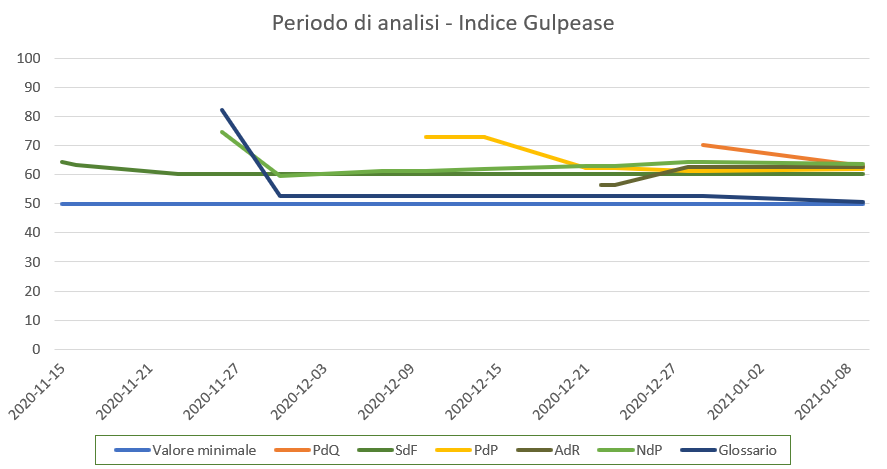
\includegraphics[scale=0.6]{Immagini/GulpeaseAnalisi}\\
	\caption{Indice di Gulpease comprendente l'andamento di tutti i documenti}
	Tutti i documenti soddisfano pienamente il valore minimo di leggibilità esposto in \hyperlink{MPR02}{MPR02}.
	\label{fig:GulpeaseAnalisi}
\end{figure}
Al termine di questo primo periodo si sono calcolati i risultati relativi alla variazione dei costi e della pianificazione. Si sono successivamente stilate due tabelle contenenti i risultati ottenuti.\\Tutti i documenti soddisfano l'obiettivo indicato in \hyperlink{MPR08}{MPR08}.
\begin{table} [H]
	\begin{center}
		\begin{tabular}{|C{6cm}|c|c|}
			\rowcolor{darkblue}
			\textcolor{white}{\textbf{Prodotto}}&
			\textcolor{white}{\textbf{Risultato ottenuto}}&
			\textcolor{white}{\textbf{Valutazione}}\\
			\NdPv{1.0.0} & 0 & Soddisfatto\\ \hline
			\SdFv{1.0.0} & 5 & Soddisfatto\\ \hline
			\AdRv{1.0.0} & 2 & Soddisfatto\\ \hline
			\PdPv{1.0.0} & 4 & Soddisfatto\\ \hline
			\PdQv{1.0.0} & 0 & Soddisfatto\\ \hline
			\Glossariov{1.0.0} & 6 & Soddisfatto\\ \hline
		\end{tabular}
	\end{center}
	\caption{\label{tab:MPR08Analisi}Risultati relativi alla varianza rispetto allo schedule.}
\end{table}\noindent
Nonostante lo sforamento di \textbf{20,00€} si è riusciti a soddisfare pienamente l'obiettivo indicato in \hyperlink{MPR09}{MPR09}.
\begin{table} [H]
	\begin{center}
		\begin{tabular}{|C{6cm}|c|c|}
			\rowcolor{darkblue}
			\textcolor{white}{\textbf{Processo}}&
			\textcolor{white}{\textbf{Risultato ottenuto}}&
			\textcolor{white}{\textbf{Valutazione}}\\
			Differenza dei costi tra il consuntivo di periodo ed il consuntivo finale & -20,00€ & Soddisfatto\\ \hline
		\end{tabular}
	\end{center}
	\caption{\label{tab:MPR09Analisi}Risultati relativi alla varianza dei costi.}
\end{table}\noindent
Nonostante le difficoltà incontrate nello svolgimento del progetto, si è riusciti a soddisfare pienamente l'obiettivo indicato in \hyperlink{MPR10}{MPR10}.
\begin{table} [H]
	\begin{center}
		\begin{tabular}{|C{6cm}|c|c|}
			\rowcolor{darkblue}
			\textcolor{white}{\textbf{Processo}}&
			\textcolor{white}{\textbf{Risultato ottenuto}}&
			\textcolor{white}{\textbf{Valutazione}}\\
			Giorni trascorsi tra l'apertura di una issue e la sua chiusura & 6 & Soddisfatto\\ \hline
		\end{tabular}
	\end{center}
	\caption{\label{tab:MPR10Analisi}Risultati relativi alla varianza dei costi.}
\end{table}

\subsection{Periodo di consolidamento dei requisiti}
In questo periodo di consolidamento dei requisiti, il gruppo {\Gruppo} si è preparato alla presentazione per la Revisione dei Requisiti studiando le varie tecnologie necessarie per l'avanzamento del progetto in modo individuale. Dal momento che non è stata eseguita nessuna operazione di verifica o miglioramento riguardante i documenti redatti, non si è ritenuto di alcuna rilevanza calcolare i risultati delle varie metriche associate alla \glo{qualità} dei documenti prodotti dal gruppo.
 
\subsection{Periodo di progettazione architetturale} \label{ResocontoPArchitetturale}
Durante il periodo di progettazione architetturale, come nel periodo precedente, i documenti redatti da presentare in ingresso alla \glo{\textbf{RP}} sono stati sottoposti a verifica secondo i criteri definiti nelle \NdPv{2.0}. In questo periodo sono stati valutati attraverso verifica anche i vari processi istanziati.
\subsubsection{Esiti verifica}
\myparagraph{Documentazione}
Di seguito si riportano gli esiti delle metriche relative alla documentazione.
\begin{figure}[h]
	\centering
	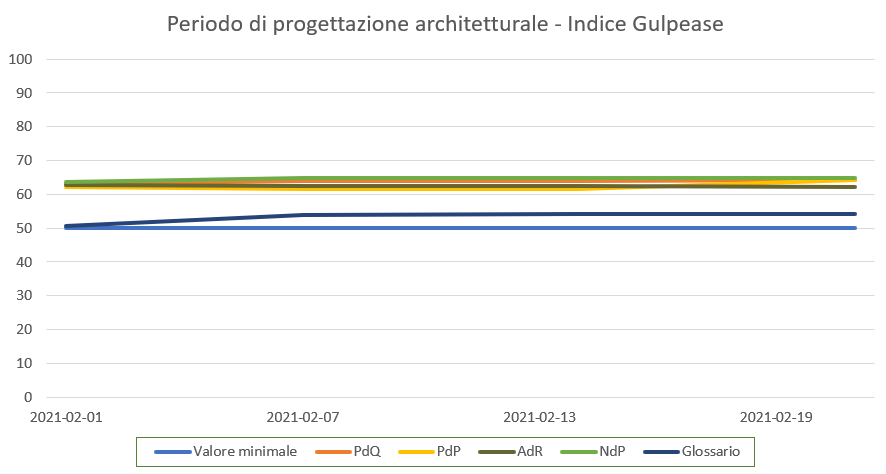
\includegraphics[scale=0.5]{Immagini/GulpeaseProgettazioneArchitetturale}\\
	\caption{Indice di Gulpease}
	\label{fig:GulpeasePArchitetturale}
\end{figure}
\begin{figure}[h]
	\centering
	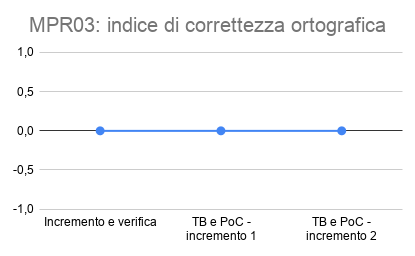
\includegraphics[scale=0.6]{Immagini/MPR03_cortografica}\\
	\caption{Correttezza ortografica documenti progettazione architetturale}
	\label{fig:CortOrtograficaPArchitetturale}
\end{figure}
\\
\myparagraph{Pianificazione}
Di seguito si riportano gli esiti delle metriche relative alla pianificazione.
\begin{figure}[h!]
	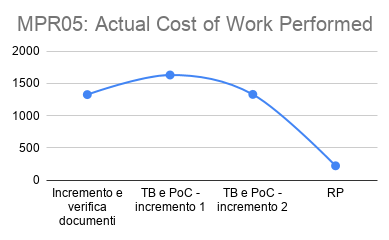
\includegraphics[scale=0.6]{Immagini/ACWP_PArchitetturale.png}\quad
	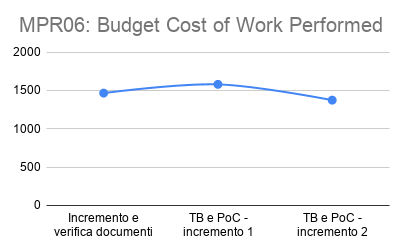
\includegraphics[scale=0.6]{Immagini/BCWP_PArchitetturale.png}
	\caption{ACWP e BCWP progettazione architetturale}
	\label{fig:BCWP_PArchitetturale}
\end{figure}
\begin{figure}[h!]
	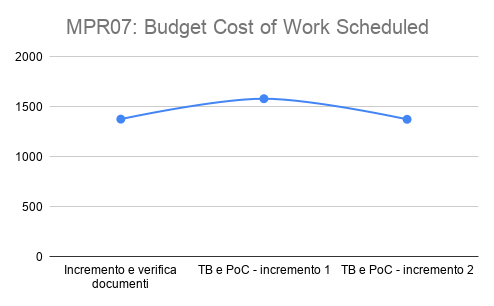
\includegraphics[scale=0.5]{Immagini/BCWS_PArchitetturale.png}\quad
 	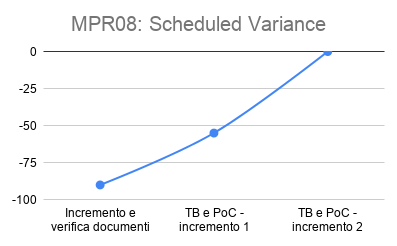
\includegraphics[scale=0.6]{Immagini/SV_PArchitetturale.png}
 	\caption{BCWS e SV progettazione architetturale}
 	\label{fig:SV_PArchitetturale}
\end{figure}
\begin{figure}[h!]
	\centering
	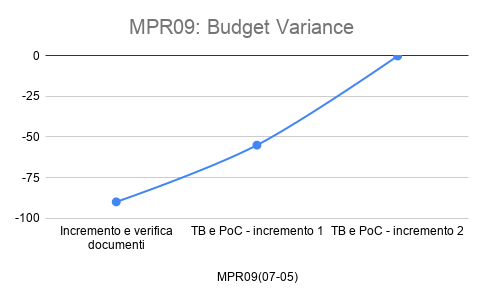
\includegraphics[scale=0.6]{Immagini/BV_PArchitetturale.png}
	\caption{BV progettazione architetturale}
	\label{fig:BV_PArchitetturale}
\end{figure}
\myparagraph{Miglioramento del processo}
Di seguito si riportano gli esiti delle metriche relative al miglioramento del processo.
\begin{figure}[h!]
	\centering
	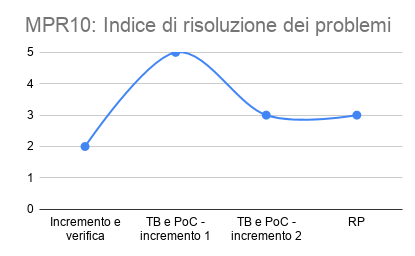
\includegraphics[scale=0.6]{Immagini/MPR10_rproblemi.png}
	\caption{Risoluzione problemi progettazione architetturale}
	\label{fig:MPR10}
\end{figure}

\subsection{Periodo di progettazione di dettaglio e codifica} \label{ResocontoPDettaglio}
Durante il periodo di progettazione di dettaglio, come nel periodo precedente, i documenti redatti da presentare in ingresso alla \glo{\textbf{RQ}} sono stati sottoposti a verifica secondo i criteri definiti nelle \NdPv{3.0}. In questo periodo sono stati valutati attraverso verifica anche i vari processi istanziati.
\newpage
\subsubsection{Esiti verifica}
\myparagraph{Documentazione}
Di seguito si riportano gli esiti delle metriche relative alla documentazione.
\begin{figure}[h]
	\centering
	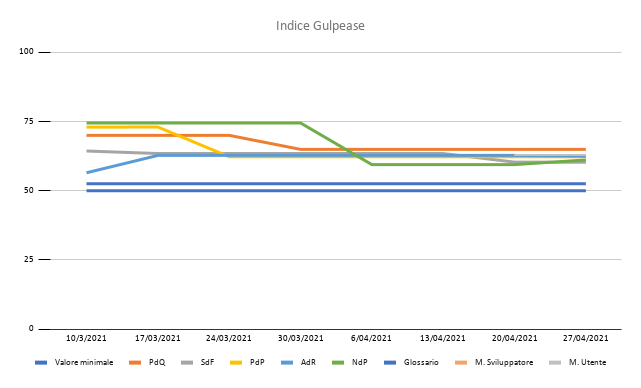
\includegraphics[scale=0.5]{Immagini/GulpeaseDettaglio}\\
	\caption{Indice di Gulpease}
	\label{fig:GulpeasePDettaglio}
\end{figure}
\begin{figure}[h]
	\centering
	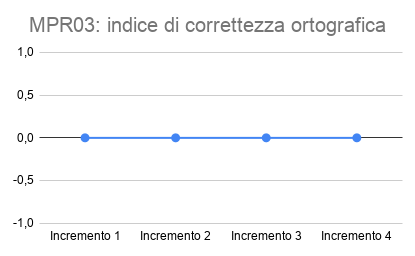
\includegraphics[scale=0.6]{Immagini/MPR03_cortograficadettaglio.png}\\
	\caption{Correttezza ortografica documenti progettazione di dettaglio e codifica}
	\label{fig:CortOrtograficaPDettaglio}
\end{figure}
\newpage
\myparagraph{Pianificazione}
Di seguito si riportano gli esiti delle metriche relative alla pianificazione.
\begin{figure}[h!]
	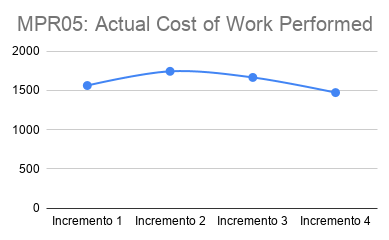
\includegraphics[scale=0.6]{Immagini/ACWP_PDettaglio.png}\quad
	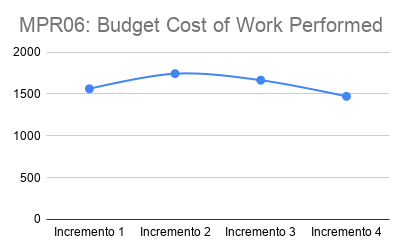
\includegraphics[scale=0.6]{Immagini/BCWP_PDettaglio.png}
	\caption{ACWP e BCWP progettazione di dettaglio e codifica}
	\label{fig:BCWP_PDettaglio}
\end{figure}
\begin{figure}[h!]
	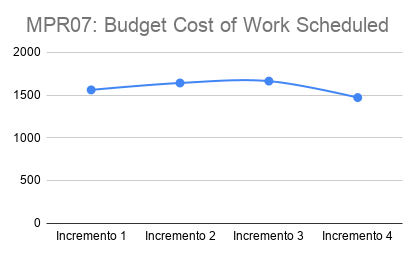
\includegraphics[scale=0.5]{Immagini/BCWS_PDettaglio.png}\quad
	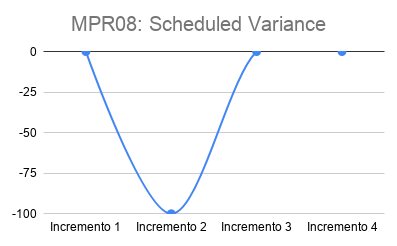
\includegraphics[scale=0.6]{Immagini/SV_PDettaglio.png}
	\caption{BCWS e SV progettazione di dettaglio e codifica}
	\label{fig:SV_PDettaglio}
\end{figure}
\begin{figure}[h!]
	\centering
	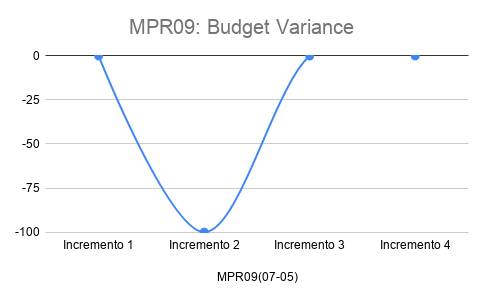
\includegraphics[scale=0.6]{Immagini/BV_PDettaglio.png}
	\caption{BV progettazione di dettaglio e codifica}
	\label{fig:BV_PDettaglio}
\end{figure}
\myparagraph{Codifica}
Di seguito si riportano gli esiti delle metriche relative alla pianificazione.
\begin{figure}[h!]
	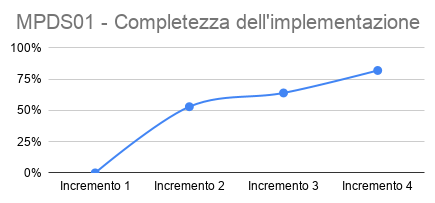
\includegraphics[scale=0.6]{Immagini/MPDS01_CompletezzaImpl.png}\quad
	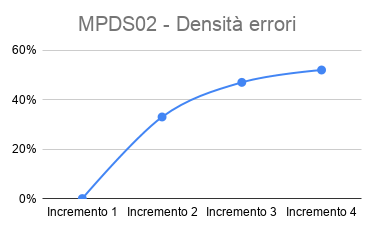
\includegraphics[scale=0.6]{Immagini/MPDS02_DErrori.png}
	\caption{Correttezza dell'implementazione e densità degli errori}
	\label{fig:DensitàErr}
\end{figure}
\begin{figure}[h!]
	\centering
	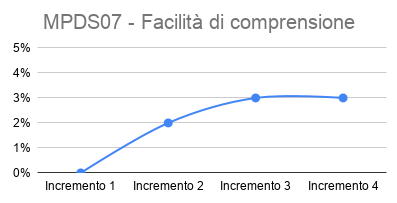
\includegraphics[scale=0.6]{Immagini/MPDS07_FComprensione.png}
	\caption{Facilità di comprensione del codice}
	\label{fig:FacilitàCodice}
\end{figure}

\myparagraph{Miglioramento del processo}
Di seguito si riportano gli esiti delle metriche relative al miglioramento del processo.
\begin{figure}[h!]
	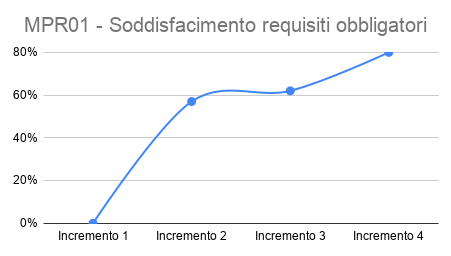
\includegraphics[scale=0.58]{Immagini/MPR01_RObbligatori.png}\quad
	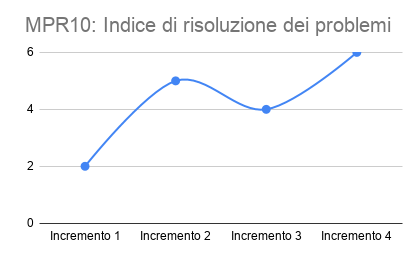
\includegraphics[scale=0.58]{Immagini/MPR10_rproblemidettaglio.png}
	\caption{Risoluzione problemi progettazione di dettaglio e codifica}
	\label{fig:MPR10codifica}
\end{figure}